\section{4D‑STEM}
{{\footnotesize
\begin{description}[labelwidth=5em, labelsep=1em, leftmargin=*, align=left, itemsep=0.3em, parsep=0em]
  \item[date:] 2023-12-03
  \item[last\_updated:] 2023-12
  \item[expired:] unkown
  \item[valid:] yes
  \item[url:] \href{https://openreview.net/pdf?id=7yt3N0o0W9}{https://openreview.net/pdf?id=7yt3N0o0W9}
  \item[domain:] Material Science
  \item[focus:] Real-time ML for scanning transmission electron microscopy
  \item[keywords:]
    - 4D-STEM
    - electron microscopy
    - real-time
    - image processing
  \item[task\_types:]
    - Image Classification
    - Streamed data inference
  \item[ai\_capability\_measured:]
    - Real-time large-scale microscopy inference
  \item[metrics:]
    - Classification accuracy
    - Throughput
  \item[models:]
    - CNN models (prototype)
  \item[ml\_motif:]
    - Real-time, Image/CV
  \item[type:] Model
  \item[ml\_task:] Image Classification
  \item[notes:] In-progress; model design under development.
  \item[contact.name:] —
  \item[contact.email:] unkown
  \item[results.name:] ChatGPT LLM
  \item[fair.reproducible:] in progress
  \item[fair.benchmark\_ready:] False
  \item[ratings.software.rating:] 0
  \item[ratings.software.reason:] Not analyzed. 
  \item[ratings.specification.rating:] 9.0
  \item[ratings.specification.reason:] Peak localization task is well-defined for diffraction images; input/output described clearly, but no system constraints.
  \item[ratings.dataset.rating:] 8.0
  \item[ratings.dataset.reason:] Simulated diffraction images provided; reusable and downloadable, but not externally versioned or FAIR-structured.
  \item[ratings.metrics.rating:] 9.0
  \item[ratings.metrics.reason:] Inference speed and localization accuracy are standard and quantitatively reported.
  \item[ratings.reference\_solution.rating:] 8.0
  \item[ratings.reference\_solution.reason:] BraggNN model and training pipeline exist, but need stitching from separate repositories.
  \item[ratings.documentation.rating:] 8.0
  \item[ratings.documentation.reason:] Paper and codebase are available and usable, though not fully turnkey.
  \item[id:] dstem
  \item[Citations:] \cite{qin2023extremely}
  \item[Ratings:]
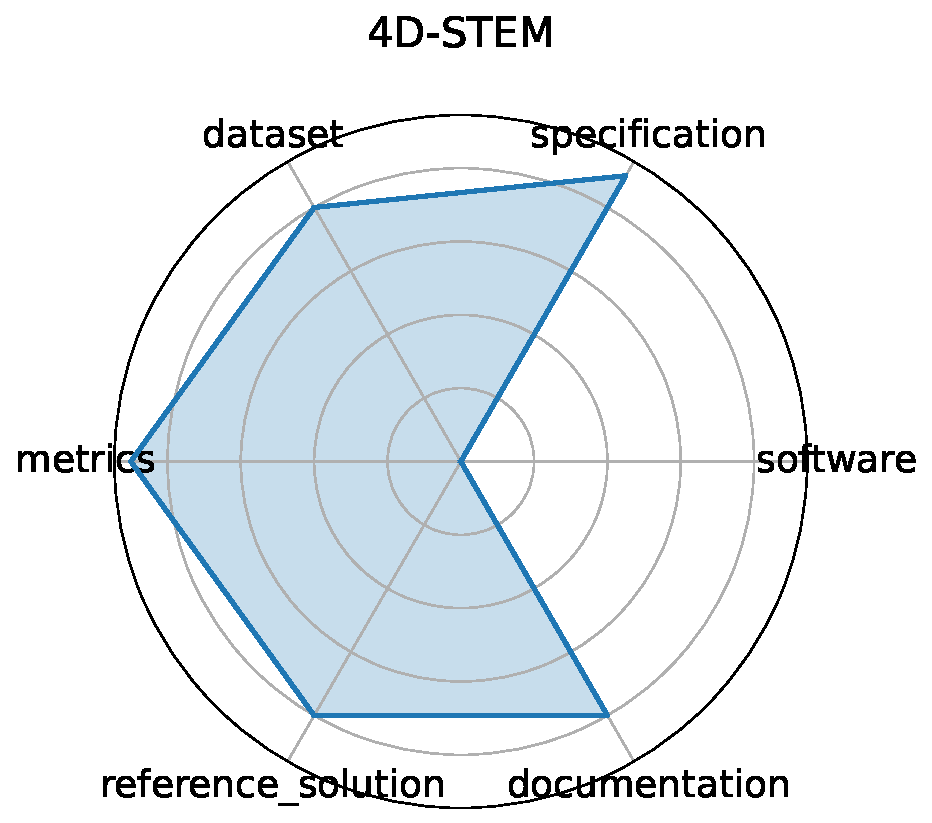
\includegraphics[width=0.2\textwidth]{dstem_radar.pdf}
\end{description}
}}
\clearpage